\documentclass{article}
% ┌─────────────────────────────────────────────────┐
% │ Packages                                        │
% └─────────────────────────────────────────────────┘

% mathematical formatting (\align, \cases, ...)
\usepackage{amsmath}

% mathematical fonts (\mathbb, \mathfrak, ...)
\usepackage{amsfonts}

% extension to amsfonts (\nexists, \square)
\usepackage{amssymb}

% theorem environments (\newtheorem)
\usepackage{amsthm}

% custom enumeration and itemize options ((i), (a), \setlist, ...)
\usepackage{enumitem}

% config management (toggles, patch commands, etc.)
\usepackage{etoolbox}

% augmented table formatting
\usepackage{multirow}

% customize section formmating
\usepackage{titlesec}

% ┌─────────────────────────────────────────────────┐
% │ Formatting Settings                             │
% └─────────────────────────────────────────────────┘

% custom theorem style: bold header (incl. parenthetical note) followed by
% a colon, with the statement itself set in normal (upright) font
\newtheoremstyle{notes}%
{\topsep}      % space above
{\topsep}      % space below
{\normalfont}  % body font (upright, not italic)
{}             % indent amount
{\bfseries}    % head font
{:}            % punctuation after head
{ }            % space after head
{\thmname{#1}\thmnumber{ #2}\thmnote{ \bfseries(#3)}}  % head spec

\theoremstyle{notes}
\newtheorem{theorem}{Theorem}
\newtheorem{lemma}[theorem]{Lemma}
\newtheorem{corollary}[theorem]{Corollary}
\newtheorem{proposition}[theorem]{Proposition}
\newtheorem{definition}[theorem]{Definition}

% removes spacing between paragraphs
\setlist{partopsep=-\parskip,parsep=0pt}

% increase text width
\setlength{\textwidth}{460pt}

% move document upwards
\setlength{\voffset}{-1cm}

% text on page before starting a new page
\setlength{\textheight}{21cm}

% increased context in error log
\setcounter{errorcontextlines}{1000}

% removes horizontal page shift
\setlength{\oddsidemargin}{0pt}

% ┌─────────────────────────────────────────────────┐
% │ Config                                          │
% └─────────────────────────────────────────────────┘

\makeatletter

\newcommand{\@@author}          {Dustin Miao}
\newcommand{\@@andrewid}        {dustinmi}
\newcommand{\@@course}          {10-783}
\newcommand{\@@section}         {A}
\newcommand{\@@duedate}         {October 08, 2026}
\newcommand{\@@hwnum}           {02}

\newtoggle{@@uselmodern}        \toggletrue{@@uselmodern}
\newtoggle{@@psetcmds}          \toggletrue{@@psetcmds}
\newtoggle{@@includefigures}    \toggletrue{@@includefigures}
\newtoggle{@@includecode}       \toggletrue{@@includecode}
\newtoggle{@@includebiblio}     \togglefalse{@@includebiblio}
\newtoggle{@@includetikz}       \togglefalse{@@includetikz}
\newtoggle{@@includeurl}        \togglefalse{@@includeurl}

\newtoggle{@@parspace}          \toggletrue{@@parspace}
\newtoggle{@@parindent}         \togglefalse{@@parindent}

\makeatother

\iffalse

\begin{table}[h]
  \centering
  \begin{tabular}{|x|x|}
    \hline
    title1 & title2 \hline
    xx & xx \\
    xx & xx \\
    \hline
  \end{tabular}
  \caption{xxxxx}
  \label{px:tab:xxxxx}
\end{table}

% figures should be stored in ./figures/
\begin{figure}[h]
  \centering
  \includegraphics[width=0.40\textwidth]{px_xxxxx}
  \caption{xxxxx}
  \label{px:fig:xxxxx}
\end{figure}

% code block
% use `style=bg' for no code highlight
\begin{minted}[opts, ...]{lang}
def main():
  print("hello world!")
\end{minted}

% code block (imported from file)
\inputminted[firstline=xx, lastline=xx]{lang}{code_file.exp}

% inline code block
\mint{lang}|print("hello world!")|

% bibliography should be stored in ./references.bib
% suggested to use bibtex entries from Google scholar w/o changing refname

\url{https://example.com}
\href{https://example.com}{Visit Example}
\href{https://example.com}{\textcolor{blue}{\uline{Visit Example}}}

\fi


\makeatletter

% redefine \maketitle command
\renewcommand{\maketitle}{
  \begin{center}
    {\huge
      Homework \@@hwnum\ Solutions
    }

    \vspace{1.5em}
    \begin{tabular}{rl}
      Author: & \@@author\ (\texttt{\@@andrewid}) \\
      Course: & \@@course\ \@@section \\
      Due by: & \@@duedate
    \end{tabular}
    \vspace{1.5em}
\end{center}}

\iftoggle{@@uselmodern}{
  % imports lmodern font
  \usepackage{lmodern}
  \renewcommand{\rmdefault}{lmss}
}{

}

\iftoggle{@@psetcmds}{
  % reformat section headers
  \titleformat{\section}
  {\normalfont\large\bfseries}
  {}
  {0pt}
  {}

  \NewDocumentCommand{\ZS}{o m}{
    \IfValueTF{#1}
    {
      \setcounter{section}{#1}
      \addtocounter{section}{-1}
    }
    {
    }
    \section{#2}
  }
}{

}

\iftoggle{@@includefigures}{
  \usepackage{graphicx}
  \graphicspath{ {./figures/} }
}{

}

\iftoggle{@@includecode}{
  \usepackage{minted}
  \usepackage{xcolor}

  \definecolor{LightGray}{gray}{0.9}
  \setminted{
    baselinestretch=1.2,
    bgcolor=LightGray,
    fontsize=\footnotesize,
    xleftmargin=14pt,
    baselinestretch=0.88,
    numbersep=4pt,
    linenos,
    mathescape,
    style=tango
  }
  \renewcommand{\theFancyVerbLine}{\ttfamily\scriptsize\arabic{FancyVerbLine}}
}{

}

\iftoggle{@@includebiblio}{
  \usepackage[
    backend=biber,
    sorting=none,
    sortcites=true,
  ]{biblatex}
  \addbibresource{references.bib}
}{

}

\iftoggle{@@includetikz}{
  \usepackage{tikz}
  \usetikzlibrary{positioning,arrows.meta}
}{

}

\iftoggle{@@includeurl}{
  \usepackage{xcolor}
  \usepackage{hyperref}
  \usepackage[normalem]{ulem}
  \usepackage{soul}
}{

}

\iftoggle{@@parspace}{
  \setlength{\parskip}{\baselineskip}
}{

}

\iftoggle{@@parindent}{
}{
  \setlength{\parindent}{0pt}
}

\makeatother

% ┌─────────────────────────────────────────────────┐
% │ Macros                                          │
% └─────────────────────────────────────────────────┘

% \mathbb
\newcommand{\bbA}{\mathbb{A}}
\newcommand{\bbB}{\mathbb{B}}
\newcommand{\bbC}{\mathbb{C}}
\newcommand{\bbD}{\mathbb{D}}
\newcommand{\bbE}{\mathbb{E}}
\newcommand{\bbF}{\mathbb{F}}
\newcommand{\bbG}{\mathbb{G}}
\newcommand{\bbH}{\mathbb{H}}
\newcommand{\bbI}{\mathbb{I}}
\newcommand{\bbJ}{\mathbb{J}}
\newcommand{\bbK}{\mathbb{K}}
\newcommand{\bbL}{\mathbb{L}}
\newcommand{\bbM}{\mathbb{M}}
\newcommand{\bbN}{\mathbb{N}}
\newcommand{\bbO}{\mathbb{O}}
\newcommand{\bbP}{\mathbb{P}}
\newcommand{\bbQ}{\mathbb{Q}}
\newcommand{\bbR}{\mathbb{R}}
\newcommand{\bbS}{\mathbb{S}}
\newcommand{\bbT}{\mathbb{T}}
\newcommand{\bbU}{\mathbb{U}}
\newcommand{\bbV}{\mathbb{V}}
\newcommand{\bbW}{\mathbb{W}}
\newcommand{\bbX}{\mathbb{X}}
\newcommand{\bbY}{\mathbb{Y}}
\newcommand{\bbZ}{\mathbb{Z}}

% \mathscr
\newcommand{\scrA}{\mathscr{A}}
\newcommand{\scrB}{\mathscr{B}}
\newcommand{\scrC}{\mathscr{C}}
\newcommand{\scrD}{\mathscr{D}}
\newcommand{\scrE}{\mathscr{E}}
\newcommand{\scrF}{\mathscr{F}}
\newcommand{\scrG}{\mathscr{G}}
\newcommand{\scrH}{\mathscr{H}}
\newcommand{\scrI}{\mathscr{I}}
\newcommand{\scrJ}{\mathscr{J}}
\newcommand{\scrK}{\mathscr{K}}
\newcommand{\scrL}{\mathscr{L}}
\newcommand{\scrM}{\mathscr{M}}
\newcommand{\scrN}{\mathscr{N}}
\newcommand{\scrO}{\mathscr{O}}
\newcommand{\scrP}{\mathscr{P}}
\newcommand{\scrQ}{\mathscr{Q}}
\newcommand{\scrR}{\mathscr{R}}
\newcommand{\scrS}{\mathscr{S}}
\newcommand{\scrT}{\mathscr{T}}
\newcommand{\scrU}{\mathscr{U}}
\newcommand{\scrV}{\mathscr{V}}
\newcommand{\scrW}{\mathscr{W}}
\newcommand{\scrX}{\mathscr{X}}
\newcommand{\scrY}{\mathscr{Y}}
\newcommand{\scrZ}{\mathscr{Z}}

% \mathcal
\newcommand{\calA}{\mathcal{A}}
\newcommand{\calB}{\mathcal{B}}
\newcommand{\calC}{\mathcal{C}}
\newcommand{\calD}{\mathcal{D}}
\newcommand{\calE}{\mathcal{E}}
\newcommand{\calF}{\mathcal{F}}
\newcommand{\calG}{\mathcal{G}}
\newcommand{\calH}{\mathcal{H}}
\newcommand{\calI}{\mathcal{I}}
\newcommand{\calJ}{\mathcal{J}}
\newcommand{\calK}{\mathcal{K}}
\newcommand{\calL}{\mathcal{L}}
\newcommand{\calM}{\mathcal{M}}
\newcommand{\calN}{\mathcal{N}}
\newcommand{\calO}{\mathcal{O}}
\newcommand{\calP}{\mathcal{P}}
\newcommand{\calQ}{\mathcal{Q}}
\newcommand{\calR}{\mathcal{R}}
\newcommand{\calS}{\mathcal{S}}
\newcommand{\calT}{\mathcal{T}}
\newcommand{\calU}{\mathcal{U}}
\newcommand{\calV}{\mathcal{V}}
\newcommand{\calW}{\mathcal{W}}
\newcommand{\calX}{\mathcal{X}}
\newcommand{\calY}{\mathcal{Y}}
\newcommand{\calZ}{\mathcal{Z}}

% \vec
\newcommand{\vva}{\vec{a}}
\newcommand{\vvb}{\vec{b}}
\newcommand{\vvc}{\vec{c}}
\newcommand{\vvd}{\vec{d}}
\newcommand{\vve}{\vec{e}}
\newcommand{\vvf}{\vec{f}}
\newcommand{\vvg}{\vec{g}}
\newcommand{\vvh}{\vec{h}}
\newcommand{\vvi}{\vec{i}}
\newcommand{\vvj}{\vec{j}}
\newcommand{\vvk}{\vec{k}}
\newcommand{\vvl}{\vec{l}}
\newcommand{\vvm}{\vec{m}}
\newcommand{\vvn}{\vec{n}}
\newcommand{\vvo}{\vec{o}}
\newcommand{\vvp}{\vec{p}}
\newcommand{\vvq}{\vec{q}}
\newcommand{\vvr}{\vec{r}}
\newcommand{\vvs}{\vec{s}}
\newcommand{\vvt}{\vec{t}}
\newcommand{\vvu}{\vec{u}}
\newcommand{\vvv}{\vec{v}}
\newcommand{\vvw}{\vec{w}}
\newcommand{\vvx}{\vec{x}}
\newcommand{\vvy}{\vec{y}}
\newcommand{\vvz}{\vec{z}}
\newcommand{\vvA}{\vec{A}}
\newcommand{\vvB}{\vec{B}}
\newcommand{\vvC}{\vec{C}}
\newcommand{\vvD}{\vec{D}}
\newcommand{\vvE}{\vec{E}}
\newcommand{\vvF}{\vec{F}}
\newcommand{\vvG}{\vec{G}}
\newcommand{\vvH}{\vec{H}}
\newcommand{\vvI}{\vec{I}}
\newcommand{\vvJ}{\vec{J}}
\newcommand{\vvK}{\vec{K}}
\newcommand{\vvL}{\vec{L}}
\newcommand{\vvM}{\vec{M}}
\newcommand{\vvN}{\vec{N}}
\newcommand{\vvO}{\vec{O}}
\newcommand{\vvP}{\vec{P}}
\newcommand{\vvQ}{\vec{Q}}
\newcommand{\vvR}{\vec{R}}
\newcommand{\vvS}{\vec{S}}
\newcommand{\vvT}{\vec{T}}
\newcommand{\vvU}{\vec{U}}
\newcommand{\vvV}{\vec{V}}
\newcommand{\vvW}{\vec{W}}
\newcommand{\vvX}{\vec{X}}
\newcommand{\vvY}{\vec{Y}}
\newcommand{\vvZ}{\vec{Z}}

% \mathbf
\newcommand{\vba}{\mathbf{a}}
\newcommand{\vbb}{\mathbf{b}}
\newcommand{\vbc}{\mathbf{c}}
\newcommand{\vbd}{\mathbf{d}}
\newcommand{\vbe}{\mathbf{e}}
\newcommand{\vbf}{\mathbf{f}}
\newcommand{\vbg}{\mathbf{g}}
\newcommand{\vbh}{\mathbf{h}}
\newcommand{\vbi}{\mathbf{i}}
\newcommand{\vbj}{\mathbf{j}}
\newcommand{\vbk}{\mathbf{k}}
\newcommand{\vbl}{\mathbf{l}}
\newcommand{\vbm}{\mathbf{m}}
\newcommand{\vbn}{\mathbf{n}}
\newcommand{\vbo}{\mathbf{o}}
\newcommand{\vbp}{\mathbf{p}}
\newcommand{\vbq}{\mathbf{q}}
\newcommand{\vbr}{\mathbf{r}}
\newcommand{\vbs}{\mathbf{s}}
\newcommand{\vbt}{\mathbf{t}}
\newcommand{\vbu}{\mathbf{u}}
\newcommand{\vbv}{\mathbf{v}}
\newcommand{\vbw}{\mathbf{w}}
\newcommand{\vbx}{\mathbf{x}}
\newcommand{\vby}{\mathbf{y}}
\newcommand{\vbz}{\mathbf{z}}
\newcommand{\vbA}{\mathbf{A}}
\newcommand{\vbB}{\mathbf{B}}
\newcommand{\vbC}{\mathbf{C}}
\newcommand{\vbD}{\mathbf{D}}
\newcommand{\vbE}{\mathbf{E}}
\newcommand{\vbF}{\mathbf{F}}
\newcommand{\vbG}{\mathbf{G}}
\newcommand{\vbH}{\mathbf{H}}
\newcommand{\vbI}{\mathbf{I}}
\newcommand{\vbJ}{\mathbf{J}}
\newcommand{\vbK}{\mathbf{K}}
\newcommand{\vbL}{\mathbf{L}}
\newcommand{\vbM}{\mathbf{M}}
\newcommand{\vbN}{\mathbf{N}}
\newcommand{\vbO}{\mathbf{O}}
\newcommand{\vbP}{\mathbf{P}}
\newcommand{\vbQ}{\mathbf{Q}}
\newcommand{\vbR}{\mathbf{R}}
\newcommand{\vbS}{\mathbf{S}}
\newcommand{\vbT}{\mathbf{T}}
\newcommand{\vbU}{\mathbf{U}}
\newcommand{\vbV}{\mathbf{V}}
\newcommand{\vbW}{\mathbf{W}}
\newcommand{\vbX}{\mathbf{X}}
\newcommand{\vbY}{\mathbf{Y}}
\newcommand{\vbZ}{\mathbf{Z}}
\newcommand{\vbmu}{\boldsymbol{\mu}}
\newcommand{\vbsigma}{\boldsymbol{\sigma}}
\newcommand{\vbSigma}{\boldsymbol{\Sigma}}
\newcommand{\vbeps}{\boldsymbol{\epsilon}}
\newcommand{\vbtau}{\boldsymbol{\tau}}

% \hat
\newcommand{\hha}{\hat{a}}
\newcommand{\hhb}{\hat{b}}
\newcommand{\hhc}{\hat{c}}
\newcommand{\hhd}{\hat{d}}
\newcommand{\hhe}{\hat{e}}
\newcommand{\hhf}{\hat{f}}
\newcommand{\hhg}{\hat{g}}
\newcommand{\hhh}{\hat{h}}
\newcommand{\hhi}{\hat{i}}
\newcommand{\hhj}{\hat{j}}
\newcommand{\hhk}{\hat{k}}
\newcommand{\hhl}{\hat{l}}
\newcommand{\hhm}{\hat{m}}
\newcommand{\hhn}{\hat{n}}
\newcommand{\hho}{\hat{o}}
\newcommand{\hhp}{\hat{p}}
\newcommand{\hhq}{\hat{q}}
\newcommand{\hhr}{\hat{r}}
\newcommand{\hhs}{\hat{s}}
\newcommand{\hht}{\hat{t}}
\newcommand{\hhu}{\hat{u}}
\newcommand{\hhv}{\hat{v}}
\newcommand{\hhw}{\hat{w}}
\newcommand{\hhx}{\hat{x}}
\newcommand{\hhy}{\hat{y}}
\newcommand{\hhz}{\hat{z}}
\newcommand{\hhA}{\hat{A}}
\newcommand{\hhB}{\hat{B}}
\newcommand{\hhC}{\hat{C}}
\newcommand{\hhD}{\hat{D}}
\newcommand{\hhE}{\hat{E}}
\newcommand{\hhF}{\hat{F}}
\newcommand{\hhG}{\hat{G}}
\newcommand{\hhH}{\hat{H}}
\newcommand{\hhI}{\hat{I}}
\newcommand{\hhJ}{\hat{J}}
\newcommand{\hhK}{\hat{K}}
\newcommand{\hhL}{\hat{L}}
\newcommand{\hhM}{\hat{M}}
\newcommand{\hhN}{\hat{N}}
\newcommand{\hhO}{\hat{O}}
\newcommand{\hhP}{\hat{P}}
\newcommand{\hhQ}{\hat{Q}}
\newcommand{\hhR}{\hat{R}}
\newcommand{\hhS}{\hat{S}}
\newcommand{\hhT}{\hat{T}}
\newcommand{\hhU}{\hat{U}}
\newcommand{\hhV}{\hat{V}}
\newcommand{\hhW}{\hat{W}}
\newcommand{\hhX}{\hat{X}}
\newcommand{\hhY}{\hat{Y}}
\newcommand{\hhZ}{\hat{Z}}

% algebra
\DeclareMathOperator{\spn}{spa}
\DeclareMathOperator{\rank}{ran}
\DeclareMathOperator{\gker}{gke}
\DeclareMathOperator{\proj}{pro}
\DeclareMathOperator{\img}{im}

% calculus
\renewcommand{\d}{\;\mathrm{d}}
\newcommand{\p}{\partial}
\newcommand{\ddx}[1]{\f{\mathrm{d}}{\mathrm{d} #1}}
\newcommand{\dydx}[2]{\f{\mathrm{d} #1}{\mathrm{d} #2}}
\newcommand{\ppx}[1]{\f{\partial}{\partial #1}}
\newcommand{\pypx}[2]{\f{\partial #1}{\partial #2}}
\newcommand{\vol}{\mathrm{vol}}

% environments
\newcommand{\BA}[1]{
  \begin{align*} #1
\end{align*}}
\newcommand{\BAC}[1]{
  \begin{align} #1
\end{align}}
\newcommand{\BC}[1]{
  \begin{cases} #1
\end{cases}}
\newcommand{\BE}[1]{
  \begin{equation*} #1
\end{equation*}}
\newcommand{\BEC}[1]{
  \begin{equation} #1
\end{equation}}
\newcommand{\BI}[1]{
  \begin{itemize}[nosep] #1
\end{itemize}}
\newcommand{\BR}[1]{
  \begin{enumerate}[label=(\roman*)] #1
\end{enumerate}}
\newcommand{\BMC}[1]{
  \begin{multline} #1
\end{multline}}
\newcommand{\BN}[1]{
  \begin{enumerate}[label=(\arabic*)] #1
\end{enumerate}}
\newcommand{\BSC}[1]{
  \begin{split} #1
\end{split}}
\newcommand{\BV}[1]{
  \begin{enumerate}[label=(\alph*)] #1
\end{enumerate}}

% groups
\newcommand{\f}[2]{\frac{#1}{#2}}
\newcommand{\bpa}[1]{\left( #1 \right)}
\newcommand{\bbb}[1]{\left[ #1 \right]}
\newcommand{\bbr}[1]{\left\{ #1 \right\}}
\newcommand{\bab}[1]{\left\lvert #1 \right\rvert}
\newcommand{\bfl}[1]{\left\lfloor #1 \right\rfloor}
\newcommand{\bcl}[1]{\left\lceil #1 \right\rceil}
\newcommand{\ban}[1]{\left\langle #1 \right\rangle}
\newcommand{\bnm}[1]{\lVert #1 \rVert}

% logic
\newcommand{\fa}{\forall}
\newcommand{\ex}{\exists}
\newcommand{\imp}{\Rightarrow}
\newcommand{\bimp}{\Leftrightarrow}

% matrices
\newcommand{\MA}[1]{
  \begin{matrix} #1
\end{matrix}}
\newcommand{\MP}[1]{
  \begin{pmatrix} #1
\end{pmatrix}}
\newcommand{\MB}[1]{
  \begin{bmatrix} #1
\end{bmatrix}}
\newcommand{\MV}[1]{
  \begin{vmatrix} #1
\end{vmatrix}}
\newcommand{\MVV}[1]{
  \begin{Vmatrix} #1
\end{Vmatrix}}

% number theory
\DeclareMathOperator{\lcm}{lc}
\DeclareMathOperator*{\argmin}{argmin}
\DeclareMathOperator*{\argmax}{argmax}

% probability
\renewcommand{\P}[1]{\mathbf{P}\left\{ #1 \right\}}
\newcommand{\E}[1]{\mathbf{E}\left[ #1 \right]}
\newcommand{\Pc}[2]{\mathbf{P}\left\{ #1 \mid #2 \right\}}
\newcommand{\Eb}{\mathbf{E}}
\newcommand{\Ec}[2]{\mathbf{E}\left[ #1 \mid #2 \right]}
\newcommand{\Ep}[2]{\mathbf{E}_{#1}\left[ #2\right]}
\newcommand{\Epc}[3]{\mathbf{E}_{#1}\left[ #2 \mid #3 \right]}
\DeclareMathOperator{\Var}{Var}
\DeclareMathOperator{\Cov}{Cov}

% values
\newcommand{\eset}{\varnothing}
\newcommand{\vZ}{\vec{0}}

\usepackage{bm}
\usepackage{twemojis}

\renewcommand{\tt}[1]{\texttt{#1}}
\newcommand{\ReLu}{\mathrm{ReLu}}
\newcommand{\oal}{\overline{\alpha}}
\newcommand{\obe}{\overline{\beta}}

\begin{document}

\maketitle

\ZS{Task 1.1}

We have that $X$ is a zero-centered Gaussian since $e^{-t}$ is a
deterministic function of time. Then, by Ito isometry,
\BE{
  \Var(X)=\E{\bpa{\int_0^2 e^{-t}\d W_t}^2}=\int_0^2 e^{-2t}\d
  t=\f{1-e^{-4}}{4}.
}
Thus, $X\sim\calN(0,(1-e^{-4})/4)$.

\ZS{Task 1.2}

Let $f(t)$ be the piecewise function
\BE{
  f(t)=\BC{1 & 0\leq t\leq 1/2 \\ 2 & 1/2 \leq t\leq 1}.
}
Because $f(t)$ is time-dependent, $X$ is a zero-centered Gaussian with variance
\BE{
  \Var(X)=\E{\bpa{\int_0^1 f(t)\d W_t}^2}=\int_0^1 f(t)^2\d t = 2.5.
}
Thus, $X\sim\calN(0,2.5)$.

\ZS{Task 1.3}

We have that
\BA{
  \Var(X)&=\E{\bpa{\int_0^1 t\d W_t}^2}=\int_0^1 t^2\d t=1/3 \\
  \Var(Y)&=\E{\bpa{\int_0^1 (1-t)\d W_t}^2}=\int_0^1 (1-t)^2\d t=1/3 \\
  \Cov(X, Y)&=\int_0^1 t(1-t)\d t=1/6.
}
This gives the joint distribution
\BE{
  \MB{X \\ Y} \sim\calN\bpa{\MB{0 \\ 0}, \MB{1/3 & 1/6 \\ 1/6 & 1/3}}.
}
Thus, $X$ and $Y$ are not independent because they have a non-zero covariance.

\ZS{Task 1.4}

Let $a,b\in \bbR$ be arbitrary reals. Then,
\BE{
  aX + bY = a\int_0^1 1\d W_t+b\int_0^1 \bpa{t-\f12}\d W_t=\int_0^1
  \bpa{a+bt-\f b2}\d W_t.
}
Since the integrand is deterministic, it follows that the
distribution of $aX+bY$ must be Gaussian, showing that the joint
distribution is Gaussian. Then,
\BE{
  \Cov(X,Y)=\int_0^1 \bpa{t-\f12}^2\d t=\left.
  \bpa{\f{t^2}{2}-\f{t}2}\right\vert_0^1=0.
}
Since the joint distribution is Gaussian and the covariance is $0$,
it follows that $X$ and $Y$ are independent.

\ZS{Task 1.5}

The integral form of Ito's formula is
\BE{
  f(W_t)-f(W_0)=\int_0^T f'(W_t)\d W_t + \f12\int_0^T f''(W_t)\d t.
}
Substituting $f(x)=x^3/3$ and rearranging gives
\BE{
  \int_0^1 W_t^2\d W_t=\f13 W_1^3 - \int_0^1 W_t\d t.
}

\ZS{Task 1.6}

\BV{
\item
  Evaluating Ito's formula with $f(x)=\f{1}{2}x^2$ in the interval
  $[0,1]$ gives
  \BE{
    \f{1}{2}W_1^2=\int_0^1 W_t\d W_t+\f12.
  }
  Rearranging and taking the expectation, we get that
  \BE{
    \E{\int_0^1 W_t\d W_t}=\E{\f{W_1^2-1}{2}}=\f{\E{W_1^2}-1}{2}=0.
  }

\item
  From Ito Isometry, we have that
  \BA{
    \E{\bpa{\int_0^1 W_t\d W_t}^2}=\E{\int_0^1 W_t^2\d t}=\int_0^1
    \E{W_t^2} \d t=\int_0^1 t\d t=1/2.
  }
}

\ZS{Task 1.7}
Consider the product rule applied to processes $W_t$ and $t$ on $[0,1]$:
\BE{
  W_1=\int_0^1 W_t\d t+\int_0^1 t\d W_t+\int_0^1 \d [W_t,t].
}
The final term on the RHS reduces to $0$, so rearranging gives the
desired result of
\BE{
  \int_0^1 t\d W_t=W_1 - \int_0^1 W_t\d t.
}
Then,
\BA{
  \Var\bpa{\int_0^1 W_t\d t}
  =\E{\bpa{\int_0^1 W_t\d t}^2}
  &=\E{\bpa{W_1-\int_0^1 t\d W_t}^2} \\
  &=\E{\bpa{\int_0^1 1\d W_t-\int_0^1 t\d W_t}^2} \\
  &=\E{\bpa{\int_0^1 (1-t)\d W_t}^2} \\
  &=\int_0^1 (1-t)^2\d t \\
  &=1/3.
}

\ZS{Task 1.8}

Let $Z=\int_a^b t\d W_t$. $Z$ is a $0$-centered Gaussian with variance
\BE{
  \Var(Z)=\E{\bpa{\int_a^b t\d W_t}^2}=\int_a^b t^2\d t=\f{1}{3}(b^3-a^3).
}
Thus, $X\sim\calN(0,1/24)$, $Y\sim\calN(0,7/24)$, and
\BE{
  X+Y=\int_0^1 t\d W_t\sim\calN(0,1/3).
}
Then, $X$ and $Y$ are independent since they are integrals of
deterministic function against Brownian increments $[0,1/2]$ and
$[1/2,1]$, which are independent.

\ZS{Task 1.9}

Since the integrand of $X_s$ is deterministic, it must have mean $0$:
$\E{X_S}=0$. Then, the covariance of $X_S$ and $X_t$ is given by
\BE{
  \Cov(X_s,X_t)=\E{\bpa{\int_0^s u\d W_u}\bpa{\int_0^t u\d
  W_u}}=\int_0^{\min(s,t)} u^2\d u=\f13(\min(s,t))^3.
}
It follows that the variance $\Var(X_t)=\f13 t^3$.

Let $s_1,\dots,s_n>0$ and $a_1,\dots,a_n\in\bbR$ be arbitrary time
points and real coefficients, respectively. Then,
\BE{
  \sum_{i=1}^n a_iX_{s_i}=\sum_{i=1}^n \bpa{a_i\int_0^{s_i} t\d
  W_t}=\int_0^1 \bpa{\sum_{i=1}^n a_i t \mathbf{1}_{t\leq s_i}}\d W_t.
}
The integrand is deterministic, so the integral must be Gaussian.
Thus, the join distribution is Gaussian, showing that
$(X_s)_{s\in[0,1]}$ is a Gaussian process.

\ZS{Task 1.10}

\BV{
\item True. Since $f\in L^2\bpa{[0,1]}$, by the Density of Step
  Function theorem, we have that for some sequence of step functions
  $f_n\in L^2\bpa([0,1])$
  \BE{
    f_n(t)=\sum_{i=0}^{k_n-1} c_i^{(n)} \mathbf{1}_{[t_i, t_{i+1}]}(t),
  }
  that $f_n\xrightarrow{L_2} f$. Define $X_n=\int_0^1 f_n(t)\d W_t$
  and $X=\int_0^1 f(t)\d W_t$. From Ito isometry,
  \BE{
    \E{(X_n-X)^2}=\E{\bpa{\int_0^1 (f_n(t)-f(t))\d
    W_t}^2}=\int_0^1 \bpa{f_n(t)-f(t)}^2\d t,
  }
  which tends to $0$ as $n\to\infty$. This shows that
  $X_n\xrightarrow{L_2}X$. Furthermore, for any $X_n$, we have that
  \BE{
    X_n=\int_0^1 f_n(t)\d W_t=\sum_{i=0}^{k_n-1}
    c_i^{(n)}(W_{t_{i+1}}-W_{t_i}).
  }
  Since $[t_i,t_{i+1}]$ interval is disjoint and Wiener process
  increments are normally distributed, this means that each $X_n$ is
  a weighted sum of independent Gaussians and is thus a Gaussian
  random variable. Since each $X_n$ is Gaussian,
  $X_n\xrightarrow{L_2}X$, and Gaussian distributions are closed
  under convergence in distribution, it follows that $X$ is also a
  Gaussian random variable, as desired.

\item
  False. For $X_t=W_t$ (adapted and in $L^2([0,1])$, the integral
    evaluates to $\f12 (W_1^2-1)$
    which is a shifted and scaled $\chi^2$ variable.

  \item
    True. For an adapted, square-integratable stochastic process $X_t$,
    the Ito integral $M_t=\int_0^t X_s\d W_t$ is a true martingale
    w.r.t. the filtration of Brownian motion. Then, by the martingale
    property, the expected value remains constant over time, so
    $\E{M_1}=\E{M_0}=0$.

  \item
    True. For any deterministic $f\in L^2([0,1])$, the Ito integral has
    mean $0$ (from part c, since any deterministic function must be
    adapted). Then, by Ito isometry,
    \BA{
      \Var\bpa{\int_0^1 f(t)\d W_t}
      &=\E{\bpa{\int_0^1 f(t)\d
      W_t}}-\E{\int_0^1 f(t)\d W_t}^2 \\
      &=\E{\bpa{\int_0^1 f(t)\d W_t}^2} \\
      &=\int_0^1 f(t)^2\d t,
    }
    as desired.
  }

  \ZS{Task 2.1}

  We have for any $\Pi_n$ that
  \BA{
    Q_{\Pi_n}(X_t)
    &=\sum_{i=0}^{n-1} (X_{t_{i+1}}-X_{t_i})^2 \\
    &=\sum_{i=0}^{n-1} (W_{t_{i+1}}-W_{t_i}+f(t_{i+1})-f(t_i))^2 \\
    &=\sum_{i=0}^{n-1} (W_{t_{i+1}}-W_{t_i})^2 + \sum_{i=0}^{n-1}
    (f(t_{i+1})-f(t_i))^2 + 2\sum_{i=0}^{n-1}
    (W_{t_{i+1}}-W_{t_i})(f(t_{i+1})-f(t_i)) \\
    \bab{Q_{\Pi_n}(X_t)-Q_{\Pi_n}(W_t)} &\leq Q_{\Pi_n}(f)
    + 2\bab{\sum_{i=0}^{n-1}
    (W_{t_{i+1}}-W_{t_i})(f(t_{i+1})-f(t_i))} \\
    &\leq Q_{\Pi_n}(f) + 2\sum_{i=0}^{n-1}
    \bab{W_{t_{i+1}}-W_{t_i}}\bab{f(t_{i+1})-f(t_i)} \\
    &\leq Q_{\Pi_n}(f) + 2\sqrt{\bpa{\sum_{i=0}^{n-1}
    (W_{t_{i+1}}-W_{t_i})^2}\bpa{\sum_{i=0}^{n-1}(f(t_{i+1})-f(t_i))^2}} \\
    &= Q_{\Pi_n}(f) + 2\sqrt{Q_{\Pi_n}(W)Q_{\Pi_n}(f)} \\
  }
  We have that $Q_{\Pi_n}(W_t)\xrightarrow{L_2} T$ and
  $Q_{\Pi_n}(f)\xrightarrow{L_2} 0$. The bound shows that
  $\left|Q_{\Pi_n}(X_t)-Q_{\Pi_n}(W_t)\right|\xrightarrow{L_2} 0$
  (since $Q_{\Pi_n}(f)$ is deterministic), so
  $Q_{\Pi_n}(X_t)\xrightarrow{L_2} T$ as well.

  \ZS{Task 2.2}

  % We show by contradiction that a strictly positive quadratic variance
  % implies that the total variance must be infinite. Assume the contrary. Then,
  % \BA{
  %   Q_{\Pi_n}(X_t)
  %   &=\sum_{i=0}^{n-1} (X_{t_{i+1}} - X_{t_i})^2 \\
  %   &=\sum_{i=0}^{n-1} \bab{X_{t_{i+1}} - X_{t_i}}^2 \\
  %   &\leq \omega_X(\Delta t)\sum_{i=0}^{n-1} \bab{X_{t_{i+1}} - X_{t_i}} \\
  %   &=\omega_X(\Delta t) \mathrm{TV}(X)
  % }
  % Assuming $X$ is almost-surely continuous, the total variation is
  % finite and the modulus of continuity tends to $0$ as $\Delta t\to 0$,
  % therefore the quadratic variation must be $0$, a contradiction.
  %
  % Since we showed in Task 2.1 that the quadratic variation is $T$ for
  % any time $T>0$, it follows that the total variation must be infinite,
  % as desired.

  We have that $W_t=X_t-f(t)$, so for each interval, we have that
  \BE{
    \bab{W_{t_{i+1}}-W_{t_i}}=\bab{(X_{t_{i+1}}-X_{t_i})+(f(t_{i+1})-f(t_i)}\leq
      \bab{X_{t_{i+1}}-X_{t_i}}+\bab{f(t_{i+1})-f(t_i}.
      }
      Summing gives
      \BE{
        \mathrm{TV}(W, [0,T])\leq \mathrm{TV}(X, [0,T]) + \mathrm{TV}(f, [0,T]).
      }
      Rearranging, we have that
      \BE{
        \mathrm{TV}(X, [0,T])\geq \mathrm{TV}(W, [0,T]) - \mathrm{TV}(f, [0,T]).
      }
      Since the total variation of a Wiener process is unbounded and
      the total variation of $f$ is finite, it follows that the total
      variation of $X$ is infinite.

      \ZS{Task 3}

      \begin{enumerate}[label=(\arabic*)]
        \item
\begin{minted}{python}
       t |    E[W_n(t)] |   theory=0 |   Var[W_n(t)] |   theory=t
  ---------------------------------------------------------------
   0.100 |     -0.00473 |      0.000 |       0.10167 |      0.100
   0.250 |     -0.00961 |      0.000 |       0.25102 |      0.250
   0.500 |     -0.01644 |      0.000 |       0.50755 |      0.500
   0.750 |     -0.02026 |      0.000 |       0.77095 |      0.750
   1.000 |     -0.02012 |      0.000 |       1.02874 |      1.000
\end{minted}

        \item
          See Figure \ref{fig:plot-paths-output}.

          \begin{figure}[h!]
            \centering
            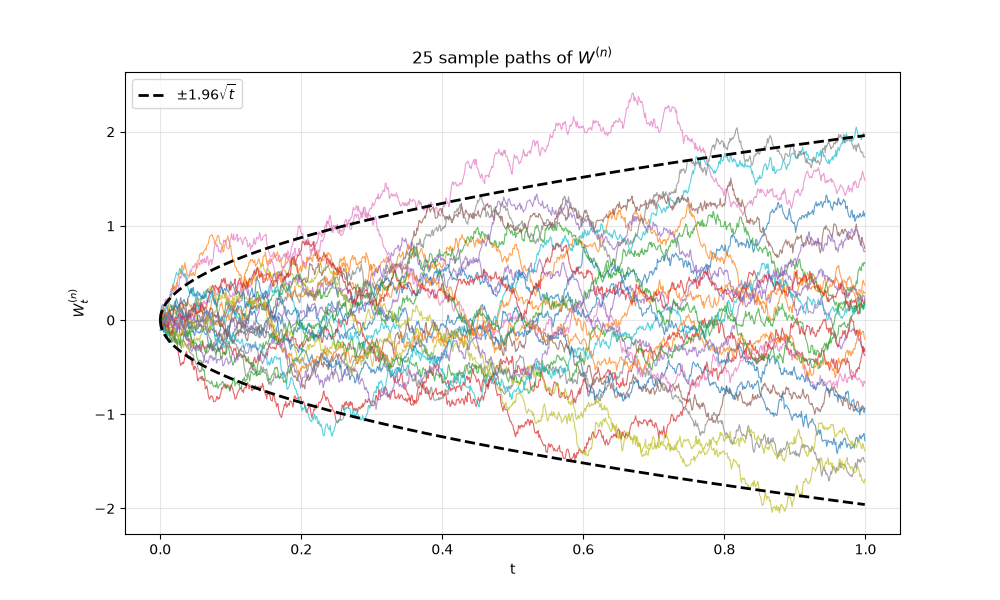
\includegraphics[width=0.75\textwidth]{plot_paths_output.png}
            \caption{25 generated Wiener processes with $95\%$ envelope}
            \label{fig:plot-paths-output}
          \end{figure}

        \item
          See Figure \ref{fig:calc-increments-output}. \\

\begin{minted}{python}
                    empirical |  theoretical
--------------------------------------------
          mean |     -0.00479 |      0.00000
      variance |      0.39814 |      0.40000
\end{minted}

          \begin{figure}[h!]
            \centering
            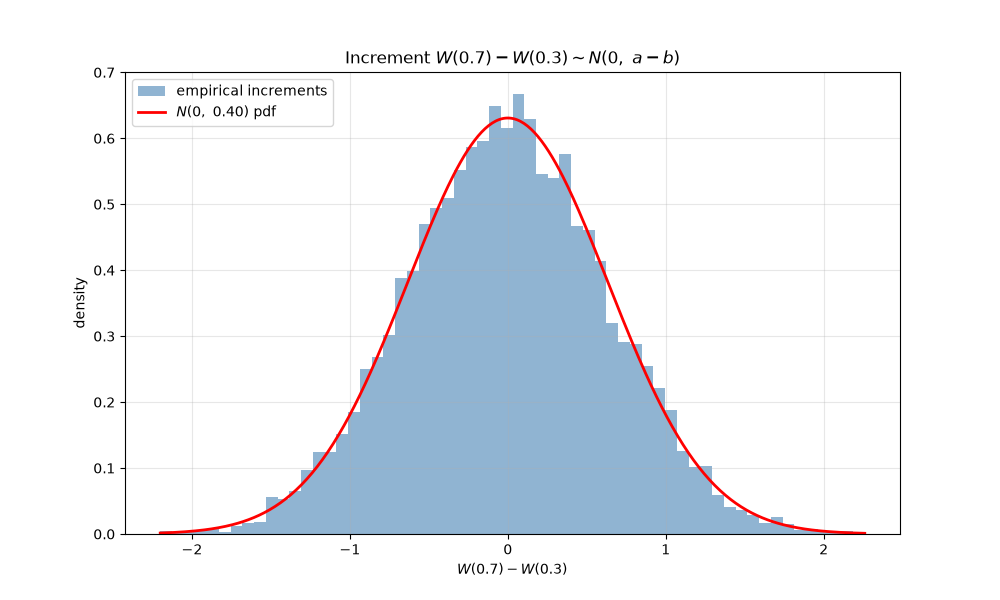
\includegraphics[width=0.75\textwidth]{calc_increments_output.png}
            \caption{Empirical distribution of Wiener process increments}
            \label{fig:calc-increments-output}
          \end{figure}

      \end{enumerate}

      \ZS{Task 4.1}

      For $I_1$, the integrand is a deterministic function of time, so it
      must be Gaussian distributed with mean $0$. The variance is given by
      Ito isometry
      \BE{
        \Var(I_1)=\E{\bpa{\int_0^1 t\d W_t}^2}=\int_0^1 t^2\d t=1/3,
      }
      giving that $I_1\sim\calN(0,1/3)$, as desired.

      \ZS{Task 4.2}

      See Figure \ref{fig:time-integral-output}. We use $m=10{,}000$
      Wiener trajectories and $n=5000$ subintervals of $[0,1]$, evaluating
      the integrand at the left endpoint. The empirical distribution is
      close to the theoretical $\calN(0,1/3)$ distribution.

      \begin{figure}[h!]
        \centering
        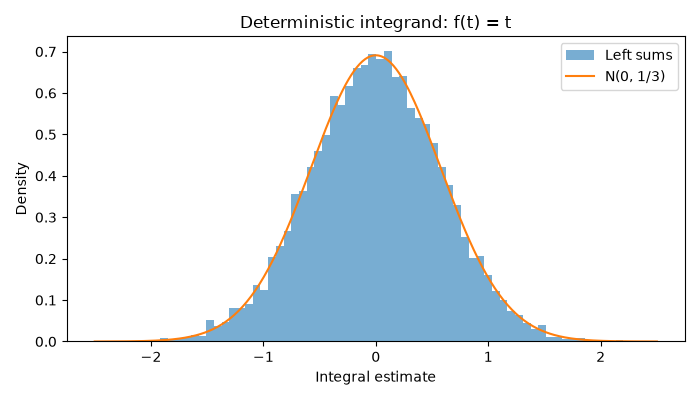
\includegraphics[width=0.75\textwidth]{time_integral_output.png}
        \caption{Empirical distribution of left tagged sums for
        $\int_0^1 t\d W_t$ with the theoretical Gaussian density}
        \label{fig:time-integral-output}
      \end{figure}

      \ZS{Task 4.3}

      See Figure \ref{fig:time-tag-differences-output}.

      \begin{figure}[h!]
        \centering
        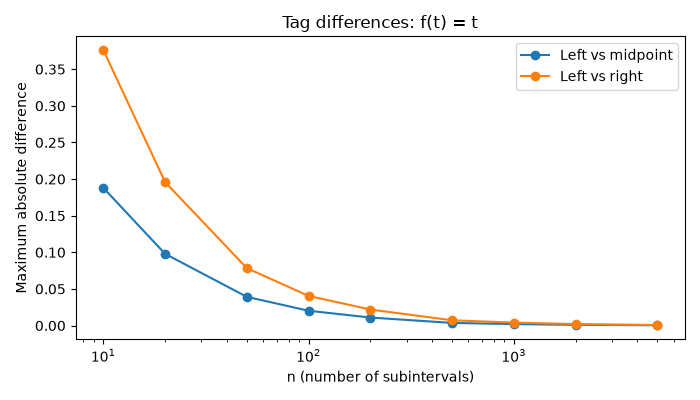
\includegraphics[width=0.75\textwidth]{time_tag_differences_output.png}
        \caption{Maximum absolute left--midpoint and left--right tag
        differences for the deterministic integrand $f(t)=t$}
        \label{fig:time-tag-differences-output}
      \end{figure}

      \ZS{Task 4.4}

      See Figure \ref{fig:wiener-integral-output}.

      \begin{figure}[h!]
        \centering
        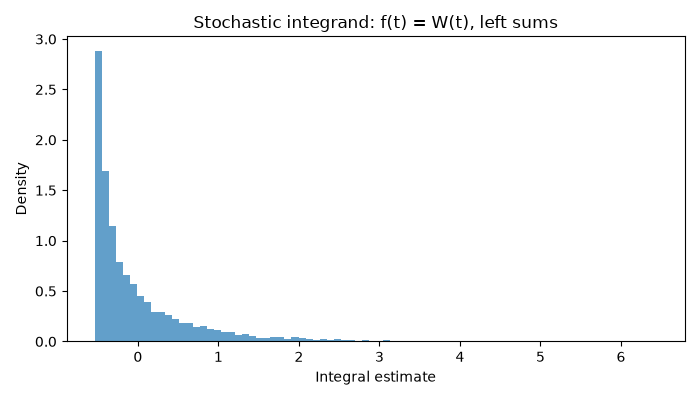
\includegraphics[width=0.75\textwidth]{wiener_integral_output.png}
        \caption{Empirical distribution of left tagged sums for
        $\int_0^1 W_t\d W_t$}
        \label{fig:wiener-integral-output}
      \end{figure}

      \ZS{Task 4.5}

      See Figure \ref{fig:wiener-tag-differences-output}. We repeat
      Task 4.3 with $f(t)=W_t$, using the same values of $n$ and $m$.
      The midpoint tags use the Brownian values at the midpoint times,
      obtained by simulating on a grid with $2n$ steps. The limits are
      \BA{
        S_n(W,\tt{left})&\to\f{W_1^2-1}{2}, \\
        S_n(W,\tt{mid})&\to\f{W_1^2}{2}, \\
        S_n(W,\tt{right})&\to\f{W_1^2+1}{2}.
      }
      The left--midpoint and left--right differences approach $1/2$
      and $1$, respectively, so the tag choice matters for this
      stochastic integrand.

      \begin{figure}[h!]
        \centering
        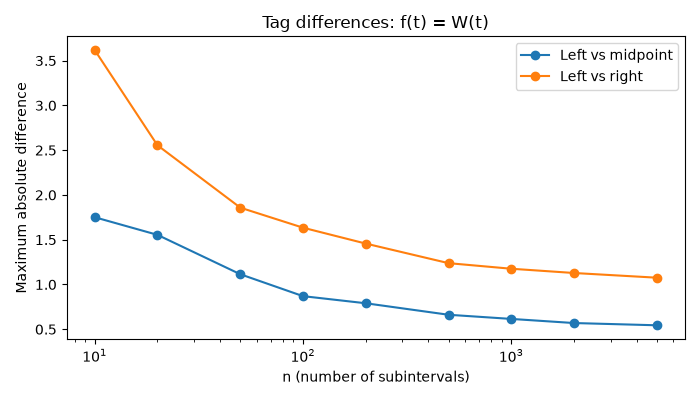
\includegraphics[width=0.75\textwidth]{wiener_tag_differences_output.png}
        \caption{Maximum absolute left--midpoint and left--right tag
        differences for the stochastic integrand $f(t)=W_t$}
        \label{fig:wiener-tag-differences-output}
      \end{figure}

      \clearpage

      \ZS{Collaboration Questions}
      \BN{
      \item
        \BV{
        \item Did you receive any help whatsoever from anyone in solving
          this assignment? No.
        \item If you answered `yes', give full details. N/A
        }
      \item
        \BV{
        \item Did you give any help whatsoever to anyone in solving this
          assignment? No.
        \item If you answered `yes', give full details. N/A.
        }
      \item
        \BV{
        \item Did you find or come across code that implements any part of
          this assignment? No.
        \item If you answered `yes', give full details. N/A
        }
      }

      \end{document}
